%%%%%%%%%%%%%%%%%%%%%%%%%%%%%%%%%%%%%%%%%
% Programming/Coding Assignment
% LaTeX Template
%
% This template has been downloaded from:
% http://www.latextemplates.com
%
% Original author:
% Ted Pavlic (http://www.tedpavlic.com)
%
% Note:
% The \lipsum[#] commands throughout this template generate dummy text
% to fill the template out. These commands should all be removed when 
% writing assignment content.
%
% This template uses a Perl script as an example snippet of code, most other
% languages are also usable. Configure them in the "CODE INCLUSION 
% CONFIGURATION" section.
%
%%%%%%%%%%%%%%%%%%%%%%%%%%%%%%%%%%%%%%%%%

%----------------------------------------------------------------------------------------
% PACKAGES AND OTHER DOCUMENT CONFIGURATIONS
%----------------------------------------------------------------------------------------

\documentclass{article}

\usepackage{fancyhdr} % Required for custom headers
\usepackage{lastpage} % Required to determine the last page for the footer
\usepackage{extramarks} % Required for headers and footers
\usepackage[usenames,dvipsnames]{color} % Required for custom colors
\usepackage{graphicx} % Required to insert images
\usepackage{listings} % Required for insertion of code
\usepackage{courier} % Required for the courier font
\usepackage{lipsum} % Used for inserting dummy 'Lorem ipsum' text into the template
\usepackage{hyperref}

% Margins
\topmargin=-0.45in
\evensidemargin=0in
\oddsidemargin=0in
\textwidth=6.5in
\textheight=9.0in
\headsep=0.25in

\linespread{1.1} % Line spacing

% Set up the header and footer
\pagestyle{fancy}
\lhead{\hmwkAuthorName} % Top left header
\chead{\hmwkClass\ (\hmwkClassInstructor\ \hmwkClassTime): \hmwkTitle} % Top center head
\rhead{\firstxmark} % Top right header
\lfoot{} % Bottom left footer
\cfoot{} % Bottom center footer
\rfoot{Page\ \thepage\ of\ \protect\pageref{LastPage}} % Bottom right footer
\renewcommand\headrulewidth{0.4pt} % Size of the header rule
\renewcommand\footrulewidth{0.4pt} % Size of the footer rule

\setlength\parindent{0pt} % Removes all indentation from paragraphs

%----------------------------------------------------------------------------------------
% CODE INCLUSION CONFIGURATION
%----------------------------------------------------------------------------------------

\definecolor{MyDarkGreen}{rgb}{0.0,0.4,0.0} % This is the color used for comments
\lstloadlanguages{Perl} % Load Perl syntax for listings, for a list of other languages supported see: ftp://ftp.tex.ac.uk/tex-archive/macros/latex/contrib/listings/listings.pdf
\lstset{language=Perl, % Use Perl in this example
        frame=single, % Single frame around code
        basicstyle=\small\ttfamily, % Use small true type font
        keywordstyle=[1]\color{Blue}\bf, % Perl functions bold and blue
        keywordstyle=[2]\color{Purple}, % Perl function arguments purple
        keywordstyle=[3]\color{Blue}\underbar, % Custom functions underlined and blue
        identifierstyle=, % Nothing special about identifiers                                         
        commentstyle=\usefont{T1}{pcr}{m}{sl}\color{MyDarkGreen}\small, % Comments small dark green courier font
        stringstyle=\color{Purple}, % Strings are purple
        showstringspaces=false, % Don't put marks in string spaces
        tabsize=5, % 5 spaces per tab
        %
        % Put standard Perl functions not included in the default language here
        morekeywords={rand},
        %
        % Put Perl function parameters here
        morekeywords=[2]{on, off, interp},
        %
        % Put user defined functions here
        morekeywords=[3]{test},
        %
        morecomment=[l][\color{Blue}]{...}, % Line continuation (...) like blue comment
        numbers=left, % Line numbers on left
        firstnumber=1, % Line numbers start with line 1
        numberstyle=\tiny\color{Blue}, % Line numbers are blue and small
        stepnumber=5 % Line numbers go in steps of 5
}

% Creates a new command to include a perl script, the first parameter is the filename of the script (without .pl), the second parameter is the caption
\newcommand{\perlscript}[2]{
\begin{itemize}
\item[]\lstinputlisting[caption=#2,label=#1]{#1.pl}
\end{itemize}
}

%----------------------------------------------------------------------------------------
% DOCUMENT STRUCTURE COMMANDS
% Skip this unless you know what you're doing
%----------------------------------------------------------------------------------------

% Header and footer for when a page split occurs within a problem environment
\newcommand{\enterProblemHeader}[1]{
\nobreak\extramarks{#1}{#1 continued on next page\ldots}\nobreak
\nobreak\extramarks{#1 (continued)}{#1 continued on next page\ldots}\nobreak
}

% Header and footer for when a page split occurs between problem environments
\newcommand{\exitProblemHeader}[1]{
\nobreak\extramarks{#1 (continued)}{#1 continued on next page\ldots}\nobreak
\nobreak\extramarks{#1}{}\nobreak
}

\setcounter{secnumdepth}{0} % Removes default section numbers
\newcounter{homeworkProblemCounter} % Creates a counter to keep track of the number of problems

\newcommand{\homeworkProblemName}{}
\newenvironment{homeworkProblem}[1][Question \arabic{homeworkProblemCounter}]{ % Makes a new environment called homeworkProblem which takes 1 argument (custom name) but the default is "Problem #"
\stepcounter{homeworkProblemCounter} % Increase counter for number of problems
\renewcommand{\homeworkProblemName}{#1} % Assign \homeworkProblemName the name of the problem
\section{\homeworkProblemName} % Make a section in the document with the custom problem count
\enterProblemHeader{\homeworkProblemName} % Header and footer within the environment
}{
\exitProblemHeader{\homeworkProblemName} % Header and footer after the environment
}

\newcommand{\problemAnswer}[1]{ % Defines the problem answer command with the content as the only argument
\noindent\framebox[\columnwidth][c]{\begin{minipage}{0.98\columnwidth}#1\end{minipage}} % Makes the box around the problem answer and puts the content inside
}

\newcommand{\homeworkSectionName}{}
\newenvironment{homeworkSection}[1]{ % New environment for sections within homework problems, takes 1 argument - the name of the section
\renewcommand{\homeworkSectionName}{#1} % Assign \homeworkSectionName to the name of the section from the environment argument
\subsection{\homeworkSectionName} % Make a subsection with the custom name of the subsection
\enterProblemHeader{\homeworkProblemName\ [\homeworkSectionName]} % Header and footer within the environment
}{
\enterProblemHeader{\homeworkProblemName} % Header and footer after the environment
}

%----------------------------------------------------------------------------------------
% NAME AND CLASS SECTION
%----------------------------------------------------------------------------------------

\newcommand{\hmwkTitle}{Assignment\ \#3} % Assignment title
\newcommand{\hmwkDueDate}{Friday,\ April\ 3,\ 2015} % Due date
\newcommand{\hmwkClass}{Introduction to Digital Libraries\ CS-751} % Course/class
\newcommand{\hmwkClassTime}{4:20pm} % Class/lecture time
\newcommand{\hmwkClassInstructor}{Michael L. Nelson} % Teacher/lecturer
\newcommand{\hmwkAuthorName}{Avinash Gosavi} % Your name

%----------------------------------------------------------------------------------------
% TITLE PAGE
%----------------------------------------------------------------------------------------

\title{
\vspace{2in}
\textmd{\textbf{\hmwkClass:\ \hmwkTitle}}\\
\normalsize\vspace{0.1in}\small{Due\ on\ \hmwkDueDate}\\
\vspace{0.1in}\large{\textit{\hmwkClassInstructor\ \hmwkClassTime}}
\vspace{3in}
}

\author{\textbf{\hmwkAuthorName}}
\date{} % Insert date here if you want it to appear below your name

%----------------------------------------------------------------------------------------


\bibliographystyle{plain}
\bibliography{reference}

\begin{document}

\maketitle

%----------------------------------------------------------------------------------------
% TABLE OF CONTENTS
%----------------------------------------------------------------------------------------

%\setcounter{tocdepth}{1} % Uncomment this line if you don't want subsections listed in the ToC

\newpage
\tableofcontents
\newpage

%----------------------------------------------------------------------------------------
% PROBLEM 1
%----------------------------------------------------------------------------------------

% To have just one problem per page, simply put a \clearpage after each problem

\begin{homeworkProblem}
For the text you saved for the 10000 URIs from A1, Q2:\\
- Use the “boilerpipe” software to remove the HTML templates from all HTML pages (document how many pages link from the tweets were non-HTML and had to be skipped)
\url{https://code.google.com/p/boilerpipe/}
WSDM 2010 paper: 
\url{http://www.l3s.de/~kohlschuetter/boilerplate/}
\\
For how many of the 10000 URIs was boilerpipe successful? \\
- Compare the total words, unique words, and byte sizes before and after use of boilerpipe\\
For what classes of pages was it successful? \\
For what classes of pages was it unsuccessful? \\
Provide examples of both successful and unsuccessful removals and discuss at length. \\
\end{homeworkProblem}

\section{Answer}

From A1, 11191 URI with response code 200 were used for A3.\

With wget data for 11,137 URI was fetched successfully.\

About 67713 unique words were found. Total size of the data was about 1.38 GB for the files downloaded.\

\subsection{Code Listing}
\subsubsection{fetchWebpages2.py}

\lstinputlisting[language=Python,breaklines = true,frame=single,caption={Before Boilerpipe}, label=lst:q1-1,captionpos=b,numbers=left,showspaces=false,showstringspaces=false,basicstyle=\footnotesize]{fetchWebpages2.py}
\newpage

With JusText data for 11062 URI was fetched successfully. But, only 4312 had content.\
About 63365 unique words were found. Total size of the data was about 26 MB for the files downloaded.\

\subsection{Code Listing}
\subsubsection{fetchWebpages.py}

\lstinputlisting[language=Python,breaklines = true,frame=single,caption={After Boilerpipe}, label=lst:q1-1,captionpos=b,numbers=left,showspaces=false,showstringspaces=false,basicstyle=\footnotesize]{fetchWebpages.py}
\newpage

\clearpage

Classes of pages that were not successful :-\\

\url{https://twitter.com/BasedMinato_/status/564132797301129216/photo/1}\

\url{http://employmentassistancesnap.com/2015/02/08/call-center-program-manager/}\

\url{http://www.weather.com/weather/today/l/26705}\\

The above pages either had lots of images instead of content or were using JavaScript to load content. With JavaScript the content is fetched later after the page is loaded by browser which Boilerpipe cannot identify because of which the files generated by Boilerpipe were empty.\\

Classes of pages that were successful :-\\

\url{http://www.smh.com.au/federal-politics/the-pulse-live/politics-live-tony-abbott-faces-liberal-leadership-spill-threat-20150209-139a1q.html.html}\

\url{http://mosaicmagazine.com/essay/2015/02/obamas-secret-iran-strategy/}\

\url{http://www.rapindustry.com/news.htm?utm_source=feedburner&utm_medium=feed&utm_campaign=Feed%3A+rapindustry%2Fhip-hop+%28Hip+Hop+Daily+news-+RAPINDUSTRY.COM%29}\\

The above pages had lots of text content which made it easier for boiler pipe to read. All content was loaded with the document load on the browser.\\

\clearpage

%----------------------------------------------------------------------------------------
% PROBLEM 2
%----------------------------------------------------------------------------------------

\begin{homeworkProblem}

Collection1: Extract all the unique terms and their frequency from the 10000 files*
Collection2: Extract all the unique terms and their frequency of the 10000 files* after running boilerpipe
Construct a table with the top 50 terms from each collection. 
Find a common stop word list.  How many of the 50 terms are on that stop word list?
For both collections, construct a graph with the x-axis as word rank, and y-axis as word frequency.  
Do either follow a Zipf distribution? Support your answer.

\end{homeworkProblem}

\section{Answer}

In next few pages there are two tables showing words given by two collections with and without boilerpipe(Only showiung 45 words because with 50 words table gets distorted).\\
The Graph for two collections is present after the tables. It clearly shows the both the collections follow Zipf distribution. Second ranked word in both list have almost half the frequency has first ranked word. And then it has a long tail for rest of the words. 

\begin{table}

\caption{  Rank,Term and Frequency before applying Boilerpipe(JusText)}

\begin{center}

  \begin{tabular}{ c | c | c }

    \hline

RANK & TERM & FREQUENCY \\ \hline
1 & the & 44622 \\ \hline
2 & and & 25270 \\ \hline
3 & to & 24455 \\ \hline
4 & of & 20162 \\ \hline
5 & a & 19400 \\ \hline
6 & in & 15115 \\ \hline
7 & is & 10787 \\ \hline
8 & for & 9272 \\ \hline
9 & that & 8938 \\ \hline
10 & you & 7857 \\ \hline
11 & on & 7063 \\ \hline
12 & with & 6528 \\ \hline
13 & it & 5994 \\ \hline
14 & are & 5406 \\ \hline
15 & this & 5315 \\ \hline
16 & i & 4912 \\ \hline
17 & was & 4888 \\ \hline
18 & as & 4747 \\ \hline
19 & have & 4523 \\ \hline
20 & be & 4240 \\ \hline
21 & at & 4136 \\ \hline
22 & or & 4057 \\ \hline
23 & not & 3931 \\ \hline
24 & by & 3777 \\ \hline
25 & from & 3660 \\ \hline
26 & he & 3652 \\ \hline
27 & we & 3373 \\ \hline
28 & your & 3346 \\ \hline
29 & will & 3262 \\ \hline
30 & his & 3192 \\ \hline
31 & an & 3041 \\ \hline
32 & has & 2983 \\ \hline
33 & but & 2910 \\ \hline
34 & they & 2832 \\ \hline
35 & if & 2719 \\ \hline
36 & their & 2473 \\ \hline
37 & all & 2455 \\ \hline
38 & can & 2276 \\ \hline
39 & new & 2254 \\ \hline
40 & who & 2237 \\ \hline
41 & more & 2120 \\ \hline
42 & about & 2060 \\ \hline
43 & one & 1986 \\ \hline
44 & so & 1978 \\ \hline
45 & out & 1809 \\ \hline

    \hline

  \end{tabular}
\end{center}
\end{table} ​

\begin{table}

\caption{  Rank,Term and Frequency From Justext File}

\begin{center}

  \begin{tabular}{ c | c | c }

    \hline

RANK & TERM & FREQUENCY \\ \hline
1 & the & 44622 \\ \hline
2 & and & 25270 \\ \hline
3 & to & 24455 \\ \hline
4 & of & 20162 \\ \hline
5 & a & 19400 \\ \hline
6 & in & 15115 \\ \hline
7 & is & 10787 \\ \hline
8 & for & 9272 \\ \hline
9 & that & 8938 \\ \hline
10 & you & 7857 \\ \hline
11 & on & 7063 \\ \hline
12 & with & 6528 \\ \hline
13 & it & 5994 \\ \hline
14 & are & 5406 \\ \hline
15 & this & 5315 \\ \hline
16 & i & 4912 \\ \hline
17 & was & 4888 \\ \hline
18 & as & 4747 \\ \hline
19 & have & 4523 \\ \hline
20 & be & 4240 \\ \hline
21 & at & 4136 \\ \hline
22 & or & 4057 \\ \hline
23 & not & 3931 \\ \hline
24 & by & 3777 \\ \hline
25 & from & 3660 \\ \hline
26 & he & 3652 \\ \hline
27 & we & 3373 \\ \hline
28 & your & 3346 \\ \hline
29 & will & 3262 \\ \hline
30 & his & 3192 \\ \hline
31 & an & 3041 \\ \hline
32 & has & 2983 \\ \hline
33 & but & 2910 \\ \hline
34 & they & 2832 \\ \hline
35 & if & 2719 \\ \hline
36 & their & 2473 \\ \hline
37 & all & 2455 \\ \hline
38 & can & 2276 \\ \hline
39 & new & 2254 \\ \hline
40 & who & 2237 \\ \hline
41 & more & 2120 \\ \hline
42 & about & 2060 \\ \hline
43 & one & 1986 \\ \hline
44 & so & 1978 \\ \hline
45 & out & 1809 \\ \hline

    \hline

  \end{tabular}
\end{center}
\end{table} ​

\clearpage

\section{Figures}

\begin{center}
\begin{figure}[ht]
    \centering
    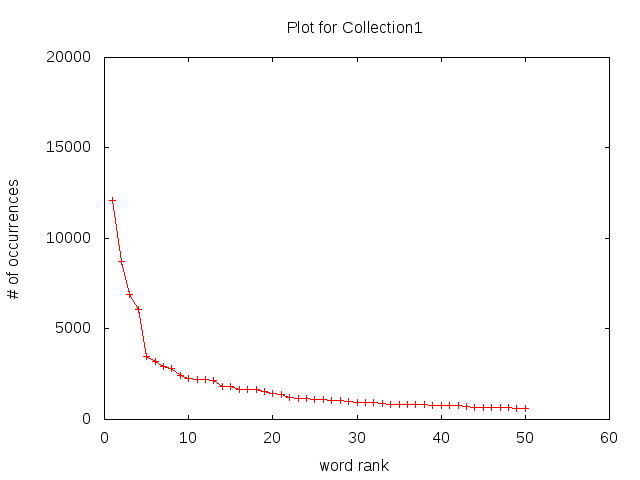
\includegraphics[width=0.475\textwidth,natwidth=700,natheight=700]{wget.png}
    \caption{Before Boilerpipe}
    \label{fig:wget.png}
\end{figure}
\end{center}

\begin{center}
\begin{figure}[ht]
    \centering
    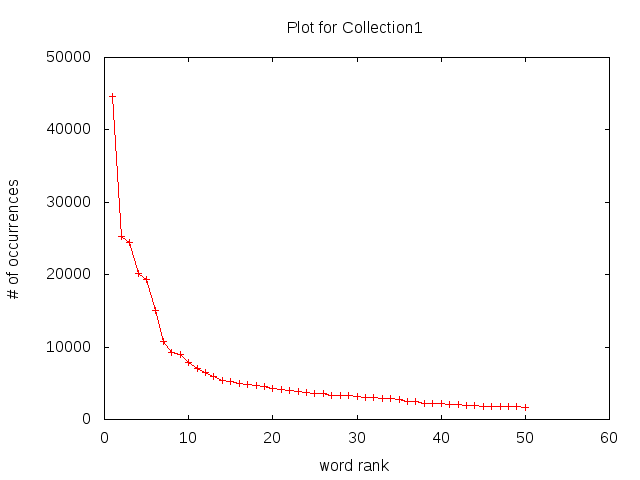
\includegraphics[width=0.475\textwidth,natwidth=700,natheight=700]{boilerpipe.png}
    \caption{After Boilerpipe}
    \label{fig:boilerpipe.png}
\end{figure}
\end{center}



%----------------------------------------------------------------------------------------

\clearpage

\end{document}